\documentclass[10pt,a4paper]{article}

\usepackage[margin=2cm]{geometry}
\usepackage[T1]{fontenc}
\usepackage{newtxtext,newtxmath}
\usepackage{microtype}
\usepackage{amsmath}
\usepackage{booktabs}
\usepackage{graphicx}
\usepackage[font=small,labelfont=bf,skip=4pt]{caption}
\usepackage[authoryear,round]{natbib}
\usepackage{multicol}
\usepackage[hyphens]{url}
\usepackage[colorlinks=true,linkcolor=black,citecolor=black,urlcolor=blue]{hyperref}
\usepackage{titlesec}

\graphicspath{{../output/figures/}}
\titlespacing*{\section}{0pt}{8pt plus 2pt}{3pt}
\titleformat{\section}{\normalfont\large\bfseries}{\thesection}{0.6em}{}
\setlength{\parskip}{2pt}
\setlength{\bibsep}{0.5pt}
\setlength{\textfloatsep}{8pt plus 2pt}
\setlength{\floatsep}{6pt plus 2pt}
\renewcommand{\arraystretch}{1.05}

% Every number below comes from the analysis scripts (analysis/*.py), which
% write these files with \newcommand. Nothing is typed by hand.
\newcommand{\NObs}{\ensuremath{330}}
\newcommand{\NCountries}{\ensuremath{21}}
\newcommand{\NBreaks}{\ensuremath{19}}
\newcommand{\NBreakCountries}{\ensuremath{11}}
\newcommand{\NKaitz}{\ensuremath{303}}
\newcommand{\NKaitzMedianCountries}{\ensuremath{14}}

\newcommand{\WithinSdMw}{\ensuremath{19}}
\newcommand{\WithinSdMwLog}{\ensuremath{0.19}}
\newcommand{\MeanIwpSal}{\ensuremath{6.3}}
\newcommand{\MeanIwp}{\ensuremath{8.4}}
\newcommand{\FrMwMaxDev}{\ensuremath{2.3}}
\newcommand{\DeMwGrowth}{\ensuremath{10}}
\newcommand{\DeMwGrowthPreHike}{\ensuremath{1}}
\newcommand{\FrIwpStart}{\ensuremath{6.3}}
\newcommand{\FrIwpEnd}{\ensuremath{6.7}}
\newcommand{\DeIwpStart}{\ensuremath{8.7}}
\newcommand{\DeIwpEnd}{\ensuremath{6.2}}
\newcommand{\DeIwpNineteen}{\ensuremath{8.1}}
\newcommand{\FrIwpTwentyOne}{\ensuremath{5.9}}
\newcommand{\FrIwpTwentyThree}{\ensuremath{6.2}}
\newcommand{\DeIwpTwentyOne}{\ensuremath{6.3}}
\newcommand{\DeBreakYears}{2019 and 2022}
\newcommand{\EsMwJump}{\ensuremath{21}}
\newcommand{\LdSlope}{\ensuremath{-0.013}}
\newcommand{\LdSe}{\ensuremath{0.013}}
\newcommand{\LdMwMax}{\ensuremath{84}}
\newcommand{\LdMwMaxCountry}{Romania}
\newcommand{\LdMwMin}{\ensuremath{-2}}
\newcommand{\RoIwpStart}{\ensuremath{18.6}}
\newcommand{\RoIwpEnd}{\ensuremath{10.7}}
\newcommand{\RoSalStart}{\ensuremath{5.8}}
\newcommand{\RoSalEnd}{\ensuremath{4.3}}
\newcommand{\RoMwGrowth}{\ensuremath{131}}
\newcommand{\RoGap}{\ensuremath{11}}
\newcommand{\OtherGap}{\ensuremath{1.3}}
\newcommand{\SurgeFr}{\ensuremath{-0.7}}
\newcommand{\SurgeMin}{\ensuremath{-11.4}}
\newcommand{\SurgeMax}{\ensuremath{+8.7}}
\newcommand{\SurgeMinCountry}{Czechia}
\newcommand{\SurgeMaxCountry}{Germany}
\newcommand{\BasketCountries}{\ensuremath{17}}
\newcommand{\BasketGapMedian}{\ensuremath{1.5}}

\newcommand{\MainB}{\ensuremath{-0.25}}
\newcommand{\MainSe}{\ensuremath{1.26}}
\newcommand{\MainPboot}{\ensuremath{0.85}}
\newcommand{\MainTen}{\ensuremath{-0.03}}
\newcommand{\MainTenLo}{\ensuremath{-0.29}}
\newcommand{\MainTenHi}{\ensuremath{+0.24}}
\newcommand{\MainLoPctMean}{\ensuremath{5}}
\newcommand{\MainMde}{\ensuremath{0.37}}
\newcommand{\MainWithinR}{\ensuremath{0.005}}
\newcommand{\MainFControlsP}{\ensuremath{0.86}}
\newcommand{\MainFYearP}{\ensuremath{0.19}}
\newcommand{\NoCtrlFYearP}{\ensuremath{0.05}}
\newcommand{\KaitzB}{\ensuremath{-0.05}}
\newcommand{\KaitzLo}{\ensuremath{-0.13}}
\newcommand{\KaitzHi}{\ensuremath{+0.03}}
\newcommand{\KaitzPboot}{\ensuremath{0.21}}
\newcommand{\KaitzMde}{\ensuremath{0.11}}
\newcommand{\AllTen}{\ensuremath{-0.16}}
\newcommand{\AllTenNoRo}{\ensuremath{+0.12}}
\newcommand{\AllKaitz}{\ensuremath{-0.13}}
\newcommand{\AllKaitzP}{\ensuremath{0.06}}
\newcommand{\AllKaitzPboot}{\ensuremath{0.11}}
\newcommand{\AllKaitzNoRo}{\ensuremath{-0.05}}
\newcommand{\MainTenNoRo}{\ensuremath{+0.05}}
\newcommand{\SimBelow}{\ensuremath{17}}
\newcommand{\SimCountries}{\ensuremath{20}}
\newcommand{\SimIncrease}{\ensuremath{16}}
\newcommand{\SimMw}{\ensuremath{0.6}}
\newcommand{\SimMwLo}{\ensuremath{6.5}}
\newcommand{\SimMwHi}{\ensuremath{5.3}}
\newcommand{\SimK}{\ensuremath{5.1}}
\newcommand{\SimKLo}{\ensuremath{13.4}}
\newcommand{\SimKHi}{\ensuremath{3.1}}

\newcommand{\BpLm}{\ensuremath{95.3}}
\newcommand{\BpDf}{\ensuremath{39}}
\newcommand{\WhiteLm}{\ensuremath{16.2}}
\newcommand{\ResSdMin}{\ensuremath{0.35}}
\newcommand{\ResSdMax}{\ensuremath{1.8}}
\newcommand{\ArRho}{\ensuremath{0.55}}
\newcommand{\FglsTen}{\ensuremath{-0.10}}
\newcommand{\FglsTenP}{\ensuremath{0.02}}
\newcommand{\FglsTenPboot}{\ensuremath{0.19}}
\newcommand{\FglsK}{\ensuremath{-0.055}}
\newcommand{\FglsKSe}{\ensuremath{0.021}}
\newcommand{\FglsKPboot}{\ensuremath{0.03}}
\newcommand{\FglsTopShare}{\ensuremath{55}}
\newcommand{\FglsNoRo}{\ensuremath{-0.01}}
\newcommand{\FglsNoIe}{\ensuremath{-0.03}}
\newcommand{\WlsTen}{\ensuremath{-0.03}}
\newcommand{\WlsK}{\ensuremath{-0.09}}
\newcommand{\WlsKPboot}{\ensuremath{0.02}}
\newcommand{\ChecksMinPboot}{\ensuremath{0.15}}
\newcommand{\LeadTen}{\ensuremath{-0.18}}
\newcommand{\LeadTenPboot}{\ensuremath{0.34}}
\newcommand{\LeadK}{\ensuremath{-0.03}}
\newcommand{\LeadKPboot}{\ensuremath{0.49}}
\newcommand{\LongRunTen}{\ensuremath{0.14}}
\newcommand{\LongRunTenP}{\ensuremath{0.45}}
\newcommand{\Elast}{\ensuremath{-0.11}}
\newcommand{\ElastSe}{\ensuremath{0.18}}
\newcommand{\QuadP}{\ensuremath{0.22}}
\newcommand{\StdMw}{\ensuremath{-0.05}}
\newcommand{\StdK}{\ensuremath{-0.15}}
\newcommand{\CookMax}{\ensuremath{0.06}}
\newcommand{\LooMin}{\ensuremath{-0.12}}
\newcommand{\LooMax}{\ensuremath{+0.05}}
\newcommand{\LooKMin}{\ensuremath{-0.07}}
\newcommand{\LooKMax}{\ensuremath{-0.03}}

\newcommand{\LineForty}{\ensuremath{-0.12}}
\newcommand{\LineFortyPct}{\ensuremath{8}}
\newcommand{\LineFortyPboot}{\ensuremath{0.07}}
\newcommand{\LineFortyMean}{\ensuremath{1.5}}
\newcommand{\LineFifty}{\ensuremath{-0.16}}
\newcommand{\LineFiftyPct}{\ensuremath{5}}
\newcommand{\LineFiftyPboot}{\ensuremath{0.12}}
\newcommand{\LineFiftyMean}{\ensuremath{3.3}}
\newcommand{\LineSixty}{\ensuremath{-0.13}}
\newcommand{\LineSixtyPct}{\ensuremath{2}}
\newcommand{\LineSixtyPboot}{\ensuremath{0.26}}
\newcommand{\LineSixtyMean}{\ensuremath{6.3}}
\newcommand{\LineSeventy}{\ensuremath{-0.21}}
\newcommand{\LineSeventyPct}{\ensuremath{2}}
\newcommand{\LineSeventyPboot}{\ensuremath{0.25}}
\newcommand{\LineSeventyMean}{\ensuremath{11.0}}
\newcommand{\MeanFt}{\ensuremath{7}}
\newcommand{\MeanPt}{\ensuremath{18}}
\newcommand{\SingleTen}{\ensuremath{-0.74}}
\newcommand{\SingleK}{\ensuremath{-0.31}}
\newcommand{\SingleKPboot}{\ensuremath{0.06}}
\newcommand{\SingleKidsTen}{\ensuremath{-0.67}}
\newcommand{\CoupleKidsTen}{\ensuremath{-0.19}}
\newcommand{\CoupleTen}{\ensuremath{-0.00}}
\newcommand{\MeanSingleKids}{\ensuremath{20}}
\newcommand{\GapTen}{\ensuremath{-0.55}}
\newcommand{\GapPboot}{\ensuremath{0.32}}
\newcommand{\ThreshElast}{\ensuremath{0.34}}
\newcommand{\ThreshElastSe}{\ensuremath{0.24}}
\newcommand{\ThreshTen}{\ensuremath{3.4}}
\newcommand{\AnchTen}{\ensuremath{-0.39}}
\newcommand{\AnchPboot}{\ensuremath{0.25}}
\newcommand{\RetTen}{\ensuremath{+0.04}}
\newcommand{\RetSe}{\ensuremath{0.39}}
\newcommand{\UneTen}{\ensuremath{+0.91}}
\newcommand{\UneSe}{\ensuremath{0.70}}
\newcommand{\EmpTen}{\ensuremath{-0.03}}
\newcommand{\EmpSe}{\ensuremath{0.60}}
\newcommand{\EmpK}{\ensuremath{-0.27}}
\newcommand{\EmpKPboot}{\ensuremath{0.21}}
\newcommand{\DeprK}{\ensuremath{0.49}}
\newcommand{\DeprKPboot}{\ensuremath{0.02}}
\newcommand{\DeprMeanWage}{\ensuremath{-3.3}}
\newcommand{\DeprMeanWageSe}{\ensuremath{0.8}}
\newcommand{\DeprMw}{\ensuremath{+1.6}}
\newcommand{\DeprMwSe}{\ensuremath{0.9}}

\newcommand{\pb}{p_{\text{boot}}}

\title{\vspace{-1.6cm}\Large\textbf{Do higher minimum wages reduce in-work poverty among employees?\\Evidence from 21 EU countries, 2009--2024}}
\author{Yuewen Sun, Victor Zacarias and Robin Herment\\[1pt]
\small Econometrics (ECO\_4MO11), T\'el\'ecom Paris, November 2026}
\date{\vspace{-0.9cm}}

\begin{document}
\maketitle

\begin{abstract}
\noindent The EU Directive on adequate minimum wages names the reduction of in-work poverty as one aim of minimum wage setting, and the simulations prepared for it predicted large falls. We study the 21 EU countries with a statutory minimum wage over income years 2009 to 2024, comparing each country with itself over time. A 10\% higher real minimum wage goes with a change of \MainTen{} percentage points in in-work poverty among employees (95\% interval \MainTenLo{} to \MainTenHi). For the increases needed to reach 50\% of the average wage, this implies a fall in in-work poverty of \SimMw\%, against 12--13\% in the simulations. The relative minimum wage (Kaitz index) has a small negative association, which becomes significant when we weight countries by their number of employees or by the precision of their data. Estimates for all workers, self-employed included, are more negative because of Romania, where poverty fell mostly outside wage employment. The poverty line seems to rise with the minimum wage, and the associations are largest for deep poverty and for single adults, which may explain the weak overall link.
\end{abstract}

\section{Introduction}

Minimum wages are now an explicit anti-poverty tool in EU policy. Directive (EU) 2022/2041 says that the setting of statutory minimum wages should be guided by criteria that aim, among other things, to reduce in-work poverty (Article 5(1)). It also asks member states to use reference values, such as 60\% of the gross median wage or 50\% of the gross average wage, to assess whether their minimum wage is adequate \citep{directive2022}. The microsimulations behind the Commission's proposal found that raising minimum wages to these values would cut in-work poverty by 12--13\% on average \citep{grunberger2021}, and an IMF study also found that a European minimum wage at 60\% of the median would reduce in-work poverty, though not overall poverty by much \citep{detragiache2020}. In November 2025 the Court of Justice annulled Article 5(2) but upheld most of the Directive \citep{cjeu2025}.

We ask whether, across the 21 EU countries with a statutory minimum wage, years with a higher real or relative minimum wage were also years with lower in-work poverty among employees, once permanent differences between countries and shocks common to all of them are held fixed. We focus on employees because the minimum wage does not cover the self-employed. We measure the minimum wage both in purchasing power and relative to the mean wage, because the poverty line is itself relative: 60\% of the national median income.

The literature does not give a clear prior. For US states, \citet{dube2019} finds that higher minimum wages raise family incomes at the bottom and reduce poverty, while \citet{neumark2005} find that they increase the share of poor and near-poor families. Studies of single European reforms point to a weak link. The German minimum wage of 2015 did little against poverty because the workers it affected are spread over the whole household income distribution \citep{backhaus2023}, and in the UK the gains of poorer working households were limited because means-tested benefits were withdrawn \citep{giupponi2024}. Comparative work adds two reasons. A full-time minimum wage keeps a single person out of poverty in only about half of the countries they study, and a one-earner couple with two children in none of them \citep{marx2012}. Wage bargaining institutions mainly shape earnings before transfers, while the benefit system affects how much in-work poverty is reduced \citep{lohmann2009}. Our contribution is after-the-fact evidence for the whole group of countries the Directive targets, which we compare directly with the simulations.

\section{Data}

All series come from the Eurostat database and were downloaded through its API by our code on 7 November 2026 \citep{eurostat2026}. The unit of observation is a country-year. The sample covers the \NCountries{} member states that had a national statutory minimum wage during the period (BE, BG, CZ, DE, EE, EL, ES, FR, HR, HU, IE, LT, LU, LV, MT, NL, PL, PT, RO, SI, SK). Austria, Denmark, Finland, Italy and Sweden have no statutory minimum wage, and Cyprus only introduced one in 2023. Germany enters in 2015.

\textbf{Outcome.} The in-work at-risk-of-poverty rate of employees aged 18--64 (table \texttt{ilc\_iw01}). Eurostat counts a person as in work if they spent at least half of the income reference year working, and as poor if the equivalised disposable income of their household is below 60\% of the national median \citep{eurostat_iw}. We also use the rate for all employed people, the rates by working time and household type (published only for all employed people), and the poverty rates of employees at lines from 40 to 70\% of the median (table \texttt{ilc\_li04}, from income year 2014).

\textbf{Timing.} EU-SILC asks about income in the previous calendar year; Ireland, the last exception in our sample, aligned in 2020 \citep{eurostat_esms}. We therefore date each observation by income year: the rate from survey wave $w$ is stored as year $w-1$ and matched with the minimum wage and controls of that year. The sample runs over income years 2009 to 2024 (waves 2010 to 2025) and has \NObs{} country-years.

\textbf{Minimum wage and controls.} We use the gross monthly statutory minimum wage (\texttt{earn\_mw\_cur}), averaged over its January and July values and deflated by each country's own HICP (2015 = 100). To compare levels across countries we express it in 2015 purchasing power standards. Within a country this is a constant factor, so it does not change any estimate with country dummies. The Kaitz index is the minimum wage as a percentage of mean gross monthly earnings (\texttt{earn\_mw\_avgr2}, \NKaitz{} observations). The controls are the unemployment rate, log real GDP per capita and the part-time share of employment. Eurostat flags \NBreaks{} breaks in the employee poverty series, in \NBreakCountries{} countries. Table~\ref{tab:desc} shows that the minimum wage moves a lot within countries: its real value varies by about \WithinSdMw\% around each country's mean, so a null result cannot come from a lack of variation.

\begin{table}[t]
\centering\footnotesize
\caption{Descriptive statistics, 21 countries, income years 2009--2024}\label{tab:desc}
\begin{tabular}{lrrrrrr}
\toprule
 & $N$ & Mean & SD & Within SD & Min & Max \\
\midrule
In-work poverty, employees (\%) & 330 & 6.3 & 2.4 & 1.0 & 2.5 & 14.7 \\
In-work poverty, all employed (\%) & 330 & 8.4 & 3.2 & 1.2 & 3.1 & 19.7 \\
Real minimum wage (2015 PPS/month) & 330 & 865.2 & 350.0 & 116.8 & 247.5 & 1641.6 \\
Kaitz index (MW / mean wage, \%) & 303 & 43.2 & 4.8 & 3.2 & 31.7 & 55.2 \\
Unemployment rate (\%) & 330 & 8.6 & 4.9 & 3.1 & 2.0 & 27.8 \\
Real GDP per capita (2020 EUR, 000s) & 330 & 27.8 & 22.4 & 4.4 & 6.9 & 107.6 \\
Part-time share of employment (\%) & 330 & 12.6 & 10.3 & 1.3 & 1.4 & 50.8 \\
\bottomrule
\end{tabular}

\\[2pt]\parbox{0.92\textwidth}{\scriptsize\textit{Note:} ``Within SD'' is the standard deviation after removing each country's mean, the only variation left once country dummies are included. The within SD of the log real minimum wage is \WithinSdMwLog. Source: Eurostat.}
\end{table}

\section{Motivating evidence}

\begin{figure}[t]
\centering
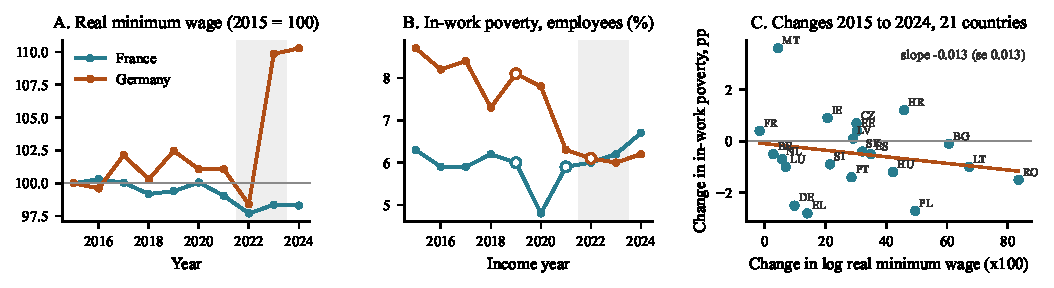
\includegraphics[width=\textwidth]{fig1_motivation.pdf}
\caption{France and Germany (A, B) and all 21 countries (C). Hollow markers are breaks in the EU-SILC series; the shaded band is the 2022--23 inflation surge. Panel C plots each country's change between income years 2015 and 2024, with the OLS line (robust standard error).}\label{fig:motivation}
\end{figure}

Figure~\ref{fig:motivation} shows why two countries are not enough. France's real minimum wage never moved more than \FrMwMaxDev\% away from its 2015 value, while Germany's was \DeMwGrowth\% higher in 2024, almost all of it after October 2022. In-work poverty among employees rose slightly in France (from \FrIwpStart\% to \FrIwpEnd\%) and fell in Germany (from \DeIwpStart\% to \DeIwpEnd\%). Most of the German fall, however, happened between 2019 and 2021 (from \DeIwpNineteen\% to \DeIwpTwentyOne\%), before the large increase, and Eurostat flags breaks in the German series in income years \DeBreakYears. Panel C uses all 21 countries. Between 2015 and 2024 the log real minimum wage changed by between \LdMwMin{} log points (France) and \LdMwMax{} (Romania), and these changes are unrelated to the changes in employee in-work poverty (slope \LdSlope, robust SE \LdSe).

Romania shows why we focus on employees. Between 2015 and 2024 in-work poverty among all its workers fell from \RoIwpStart\% to \RoIwpEnd\%, while among employees it went from \RoSalStart\% to \RoSalEnd\%. Most of the fall therefore happened outside wage employment, although the real minimum wage rose by \RoMwGrowth\%. On average the gap between the two rates is \RoGap{} points in Romania and \OtherGap{} points in the median of the other countries.

\section{Empirical strategy}

We estimate
\begin{equation}
\mathit{IWP}_{it} = \beta\, \mathit{MW}_{it} + X_{it}'\gamma + \alpha_i + \delta_t + u_{it},
\label{eq:main}
\end{equation}
where $\mathit{IWP}_{it}$ is the in-work poverty rate (percentage points) of country $i$ in income year $t$, $\mathit{MW}_{it}$ is either the log real minimum wage or the Kaitz index, $X_{it}$ holds the controls, and $\alpha_i$ and $\delta_t$ are country and year dummies (one of each is dropped to avoid the dummy variable trap). The country dummies absorb everything that is permanent about a country, such as the broad design of its benefit system or its family structure, so $\beta$ is estimated only from changes within countries over time: the German increase of 2022, the \EsMwJump\% real increase in Spain in 2019, or the repeated increases in Romania and Bulgaria. The year dummies absorb shocks common to all countries, such as COVID or the energy prices of 2022. With the log real minimum wage, $\beta/10$ is approximately the change in percentage points for a 10\% higher minimum wage (level-log form).

Reading $\beta$ as a causal effect requires strict exogeneity, $E(u_{it}\mid \mathit{MW}_{i1},\dots,\mathit{MW}_{iT}, X_{i1},\dots,X_{iT}, \alpha_i)=0$ \citep[ch.~13--14]{wooldridge2013}. Minimum wage changes must not react to past or expected shocks to poverty, and they must not come together with other country-specific changes such as tax and benefit reforms. We cannot guarantee either with observational data, so we read $\beta$ as a conditional association and test one implication of strict exogeneity with a lead of the minimum wage (Section~\ref{sec:robust}).

The residuals of \eqref{eq:main} are heteroskedastic (Breusch--Pagan LM $=\BpLm$ with \BpDf{} degrees of freedom, $p<0.001$; special White test $p<0.001$). Their standard deviation goes from \ResSdMin{} points in Belgium and the Netherlands to \ResSdMax{} in Hungary. They are also autocorrelated within countries (first-order coefficient \ArRho). We therefore cluster standard errors by country, which allows for any heteroskedasticity and any correlation within a country, and use the $t$ distribution with 20 degrees of freedom. With only 21 clusters the cluster-robust test can still reject too often \citep{cameron2015}, so for every coefficient of interest we also report a wild cluster bootstrap $p$-value ($\pb$; restricted residuals, Webb six-point weights, 9{,}999 draws) following \citet{cameron2008} and \citet{webb2023}.

\section{Results}

\begin{table}[t]
\centering\footnotesize
\caption{Minimum wage and in-work poverty: from pooled OLS to two-way fixed effects}\label{tab:main}
\setlength{\tabcolsep}{4.5pt}
\begin{tabular}{lcccccccc}
\toprule
 & \multicolumn{6}{c}{Employees} & \multicolumn{2}{c}{All employed} \\
\cmidrule(lr){2-7}\cmidrule(lr){8-9}
 & (1) & (2) & (3) & (4) & (5) & (6) & (7) & (8) \\
\midrule
Log real minimum wage & $-0.46$ & $-0.33$ & $-0.14$ & $-0.25$ &  & $0.15$ & $-1.58$ &  \\
 & $(1.22)$ & $(1.05)$ & $(1.28)$ & $(1.26)$ &  & $(1.72)$ & $(2.08)$ &  \\
 & $[0.75]$ & $[0.77]$ & $[0.91]$ & $[0.85]$ &  & $[0.94]$ & $[0.64]$ &  \\[2pt]
Kaitz index (points) &  &  &  &  & $-0.05$ & $-0.05$ &  & $-0.13^{*}$ \\
 &  &  &  &  & $(0.04)$ & $(0.06)$ &  & $(0.07)$ \\
 &  &  &  &  & $[0.21]$ & $[0.41]$ &  & $[0.11]$ \\[2pt]
\midrule
Country dummies & No & Yes & Yes & Yes & Yes & Yes & Yes & Yes \\
Year dummies & No & No & Yes & Yes & Yes & Yes & Yes & Yes \\
Controls & No & Yes & No & Yes & Yes & Yes & Yes & Yes \\
Observations & 330 & 330 & 330 & 330 & 303 & 303 & 330 & 303 \\
Within $R^2$ &  & 0.018 & 0.000 & 0.005 & 0.023 & 0.023 & 0.056 & 0.126 \\
$F$ test, year dummies ($p$) &  &  & 0.05 & 0.19 & 0.09 & 0.08 & 0.00 & 0.02 \\
\bottomrule
\end{tabular}

\\[2pt]\parbox{0.96\textwidth}{\scriptsize\textit{Note:} Dependent variable: in-work poverty rate (pp) of employees in (1)--(6) and of all employed people in (7)--(8). Standard errors clustered by country in parentheses; wild cluster bootstrap $p$-values in brackets. $^{*}p<0.1$, $^{**}p<0.05$, $^{***}p<0.01$ (clustered $t$ test, 20 degrees of freedom). Controls: unemployment rate, log real GDP per capita, part-time share. Columns (5), (6) and (8) use the \NKaitz{} observations with a Kaitz index.}
\end{table}

Table~\ref{tab:main} goes from a pooled regression across countries to the full model. All estimates for employees are small and far from significant. In the main specification, column (4), the coefficient is \MainB{} (SE \MainSe, $\pb=\MainPboot$): a 10\% higher real minimum wage goes with a change of \MainTen{} points in in-work poverty, with a 95\% interval from \MainTenLo{} to \MainTenHi. Since the mean is \MeanIwpSal\%, the interval rules out reductions larger than about \MainLoPctMean\% of the mean, and the minimum detectable effect at 80\% power is \MainMde{} points per 10\%. The regressors explain almost none of the variation within countries (within $R^2=\MainWithinR$), and the controls are jointly insignificant ($p=\MainFControlsP$). The Kaitz index gives a similar answer: \KaitzB{} points per Kaitz point (interval \KaitzLo{} to \KaitzHi, $\pb=\KaitzPboot$). Including both measures in column (6) changes nothing.

\begin{figure}[t]
\centering
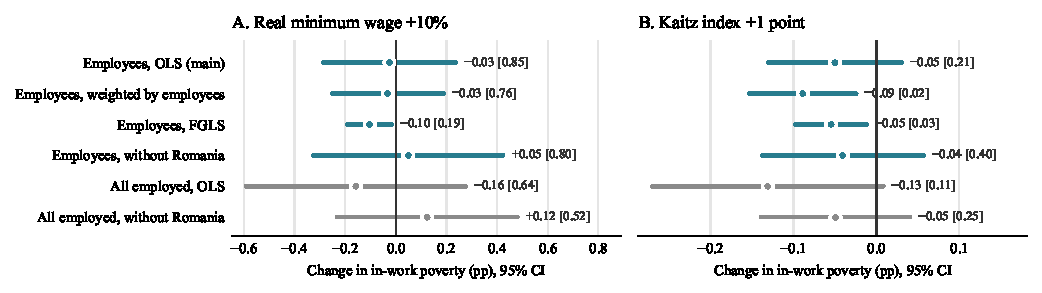
\includegraphics[width=0.93\textwidth]{fig2_estimates.pdf}
\caption{Change in in-work poverty (pp) for a 10\% higher real minimum wage (A) or a one-point higher Kaitz index (B), two-way FE with controls. Lines are 95\% intervals from country-clustered standard errors; wild cluster bootstrap $p$-values in brackets. WLS weights each country-year by its number of employees; FGLS by the inverse of the country's residual variance.}\label{fig:estimates}
\end{figure}

OLS gives every country-year the same weight, although some poverty series are much noisier than others. Figure~\ref{fig:estimates} adds two weighted estimators: WLS with the number of employees as weights, which describes the average employee rather than the average country, and feasible GLS (FGLS), which weights each country by the inverse of its residual variance. For the Kaitz index both are negative and significant (\WlsK, $\pb=\WlsKPboot$, and \FglsK, $\pb=\FglsKPboot$). For the real minimum wage, FGLS gives \FglsTen{} per 10\% with a clustered $p$-value of \FglsTenP{} but a bootstrap $p$-value of \FglsTenPboot. Four countries get \FglsTopShare\% of the weight, so in effect there are few clusters, which is when the usual test rejects too often; without Romania the estimate falls to \FglsNoRo. For all employed people, columns (7) and (8) are more negative, but Figure~\ref{fig:estimates} shows that this comes from Romania. Without it they move to \AllTenNoRo{} per 10\% and \AllKaitzNoRo{} per Kaitz point, while the estimates for employees barely change.

These estimates can be compared with the simulations. In 2019, \SimBelow{} of the \SimCountries{} countries with data had a minimum wage below 50\% of the average wage, and reaching that level would have required an increase of \SimIncrease\% on average. Our main coefficient implies that this would lower employee in-work poverty by \SimMw\% on average (95\% interval: a fall of \SimMwLo\% to a rise of \SimMwHi\%), far from the 12--13\% of \citet{grunberger2021}. With the Kaitz index the implied fall is \SimK\% (a fall of \SimKLo\% to a rise of \SimKHi\%), so the simulated value is at the edge of the interval. The simulations give first-round effects for all workers with most behaviour held fixed, while our estimates include whatever adjustments happened in practice.

\section{Robustness and mechanisms}\label{sec:robust}

\begin{table}[t]
\centering\footnotesize
\caption{Robustness checks and other outcomes (two-way FE with controls)}\label{tab:checks}
\setlength{\tabcolsep}{5pt}
\begin{tabular}{lccccc}
\toprule
 & \multicolumn{2}{c}{Real minimum wage $+10\%$} & \multicolumn{2}{c}{Kaitz index $+1$ point} & \\
\cmidrule(lr){2-3}\cmidrule(lr){4-5}
 & Effect (SE) & $p_{\text{boot}}$ & Effect (SE) & $p_{\text{boot}}$ & $N$ \\
\midrule
\multicolumn{6}{l}{\textit{A. Robustness. Outcome: in-work poverty of employees (pp)}} \\
No controls & $-0.01$ (0.13) & 0.91 & $-0.03$ (0.04) & 0.37 & 330 \\
Separate level after each series break & $+0.13$ (0.17) & 0.50 & $-0.04$ (0.04) & 0.37 & 330 \\
Minimum wage of the survey year & $-0.05$ (0.12) & 0.72 & $-0.05$ (0.04) & 0.16 & 331 \\
Without income years 2020--21 & $-0.03$ (0.14) & 0.81 & $-0.06$ (0.04) & 0.16 & 288 \\
Without Romania & $+0.05$ (0.18) & 0.80 & $-0.04$ (0.05) & 0.40 & 314 \\
Deflated by low-income (Q1) prices & $-0.02$ (0.11) & 0.85 &  &  & 330 \\
Kaitz index on the median wage &  &  & $0.00$ (0.06) & 0.96 & 147 \\
First differences within segments & $-0.04$ (0.10) & 0.66 & $-0.01$ (0.04) & 0.80 & 290 \\
WLS, weights = number of employees & $-0.03$ (0.11) & 0.76 & $-0.09$ (0.03) & 0.02 & 330 \\
FGLS, weights = 1 / country residual variance & $-0.10$ (0.04) & 0.19 & $-0.05$ (0.02) & 0.03 & 330 \\
Placebo: next year's minimum wage (lead) & $-0.18$ (0.18) & 0.34 & $-0.03$ (0.05) & 0.49 & 329 \\
\midrule
\multicolumn{6}{l}{\textit{B. Other outcomes (sample mean in parentheses)}} \\
Log real poverty line$^{a}$ & $+0.34$ (0.24) & 0.33 & $0.00$ (0.01) & 0.96 & 330 \\
Poverty, line anchored at its 2008 value$^{b}$ (13) & $-0.39$ (0.23) & 0.25 & $0.00$ (0.14) & 0.99 & 314 \\
Poverty of retired people (placebo)$^{c}$ (20) & $+0.04$ (0.39) & 0.93 & $+0.05$ (0.20) & 0.84 & 230 \\
Employment rate, low education$^{d}$ (51) & $-0.03$ (0.60) & 0.97 & $-0.27$ (0.18) & 0.21 & 330 \\
Material deprivation, bottom quintile$^{b}$ (39) & $-1.40$ (0.95) & 0.30 & $+0.49$ (0.18) & 0.02 & 230 \\
\bottomrule
\end{tabular}

\\[2pt]\parbox{0.96\textwidth}{\scriptsize\textit{Note:} Each row is a separate regression of model \eqref{eq:main}, with standard errors clustered by country. $^{a}$Elasticity of the real poverty line with respect to the real minimum wage (coefficient on the log, not divided by 10). $^{b}$Whole population aged 18--64 (anchored line) or bottom income quintile (deprivation, dated by survey year). $^{c}$Retired people aged 18 and over, income years 2014--2024. $^{d}$Employment rate (\%) of people aged 20--64 with at most lower secondary education.}
\end{table}

None of the checks in panel~A of Table~\ref{tab:checks} moves the employee estimates far from zero, and apart from the weighted estimators none has $\pb$ below \ChecksMinPboot. This includes dropping the controls, which could themselves respond to the minimum wage, and estimating in first differences. Deflating by a price index built from the budget shares of the poorest fifth of households gives the same result, although their prices rose faster than those of the richest fifth in \BasketCountries{} of the 21 countries between 2020 and 2024. In a distributed-lag model, next year's minimum wage does not predict this year's poverty (\LeadTen{} per 10\%, $\pb=\LeadTenPboot$), so we see no sign of the feedback that would violate strict exogeneity, although the test has little power. Dropping one country at a time keeps the main estimate between \LooMin{} and \LooMax{} per 10\%, and no country-year dominates the fit (largest Cook's distance \CookMax). With the outcome in logs the elasticity is \Elast{} (SE \ElastSe), and a quadratic in the Kaitz index adds nothing (joint $F$ test $p=\QuadP$).

Panel~B first checks two concerns. Poverty among retired people, whose income does not depend on the minimum wage, does not move with it either (\RetTen{} per 10\%, SE \RetSe), so we find no sign of a general fall in poverty in years with high minimum wages. The employment rate of people with at most lower secondary education does not fall either (\EmpTen{} points per 10\%, SE \EmpSe), so we see no sign that low-paid workers were pushed out of our sample.

\begin{figure}[t]
\centering
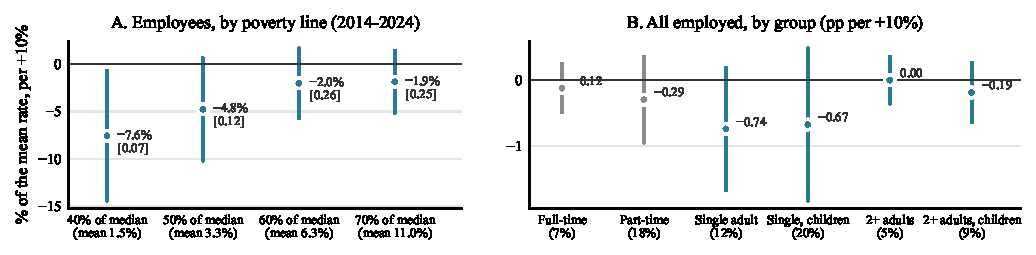
\includegraphics[width=0.93\textwidth]{fig3_mechanisms.pdf}
\caption{(A) Change in the poverty rate of employees aged 18 and over (table \texttt{ilc\_li04}) for a 10\% higher real minimum wage, as a percentage of the mean rate, at four poverty lines; income years 2014--2024. (B) Change in in-work poverty of all employed people by working time and household type, pp per 10\%, sample means in parentheses. Two-way FE with controls; 95\% intervals from clustered standard errors; bootstrap $p$-values in brackets (A).}\label{fig:mechanisms}
\end{figure}

Three results help explain the weak link. First, the poverty line seems to move with the minimum wage. A 10\% higher real minimum wage goes with a \ThreshTen\% higher real poverty line, although the elasticity of \ThreshElast{} is imprecise (SE \ThreshElastSe). If so, part of any gain at the bottom is matched by a higher line, and indeed poverty measured against a line fixed at its 2008 real value responds more (\AnchTen{} points per 10\%, $\pb=\AnchPboot$). Second, the minimum wage seems to matter more for deep poverty (Figure~\ref{fig:mechanisms}A). Relative to its mean, poverty below 40\% of the median is \LineFortyPct\% lower when the minimum wage is 10\% higher ($\pb=\LineFortyPboot$), against \LineFiftyPct\% below 50\% and about \LineSixtyPct\% below the 60\% and 70\% lines. One reading is that a higher minimum wage lifts some workers out of deep poverty without taking them above the official line. Third, household composition seems to matter (Figure~\ref{fig:mechanisms}B). The largest associations are for single adults (\SingleTen{} points per 10\%; \SingleK{} per Kaitz point, $\pb=\SingleKPboot$), whose household lives on one wage, and the smallest are for couples, who often have a second income. Most minimum wage earners in fact live with another adult and are not concentrated in the poorest households \citep{eurofound2024}. The gap between single adults and couples with children is not significant, though (\GapTen{} per 10\%, $\pb=\GapPboot$). Part-time workers are poor far more often than full-time workers (\MeanPt\% against \MeanFt\%), as in \citet{horemans2016}, but both estimates are imprecise. Since we test many outcomes, a few $p$-values near 0.05 can appear by chance, and we read these patterns as suggestive.

Finally, a higher Kaitz index goes with more material deprivation in the bottom income quintile (\DeprK, $\pb=\DeprKPboot$). Splitting the index shows why: deprivation falls when the real mean wage rises (\DeprMeanWage{} points per 10\%, SE \DeprMeanWageSe) and is not significantly related, at 5\%, to the minimum wage itself (\DeprMw{} per 10\%, SE \DeprMwSe). The index also rises when average pay falls in bad years, so a change in it is not always a change in policy.

\section{Limitations and conclusion}

Our estimates are conditional associations. Minimum wages respond to economic conditions and politics, other policies change at the same time, and the dummies do not remove country-specific shocks. Aggregate rates hide who earns the minimum wage and in which household. We also observe gross rather than net pay: Romania raised its gross minimum wage by 52\% between January 2017 and January 2018, but the 2018 step compensated workers for social contributions that were moved from employers to employees \citep{eurofound2018}. Two-way fixed effects can also weight effects that differ across countries and years in odd ways, even negatively \citep{dechaisemartin2020}.

Over 2009 to 2024, years with a higher real minimum wage were not years with lower in-work poverty among employees, and the relative minimum wage has at most a small negative association. Both are smaller than the reductions in the simulations and agree with the after-the-fact studies of Germany and the UK. France illustrates this. With automatic indexation \citep{eurofound2024}, its real minimum wage changed by only \SurgeFr\% over 2021 to 2023, while other countries ranged from \SurgeMin\% in \SurgeMinCountry{} to \SurgeMax\% in \SurgeMaxCountry, yet in-work poverty among French employees went from \FrIwpTwentyOne\% to \FrIwpTwentyThree\%. Our mechanism estimates are imprecise, but they point to the relative poverty line and to household composition, and suggest that the minimum wage matters more for deep poverty. Like \citet{marx2012}, we conclude that the minimum wage alone can do only so much against in-work poverty.

\vspace{3pt}
{\small\noindent\textbf{Code and data.} All results can be reproduced with \texttt{python run\_all.py} from our repository, which includes the Eurostat snapshot used here and a notebook (\texttt{analysis.ipynb}) with every step and its output: \url{https://github.com/VictorZaca/minimum-wages-in-work-poverty-eu}.
\textbf{Contributions.} Yuewen Sun and Robin Herment prepared the project proposal. Yuewen led the France and Germany comparison and the motivating evidence, Robin led the policy background and the literature, and Victor Zacarias led the data work, the code and the regressions. All three of us discussed the specification, wrote and revised the report, and prepared the slides and the presentation together.
\textbf{Use of AI.} We used an AI assistant (Claude, Anthropic) to help write and check the code, find and check references, and edit the English. We checked the sources and results ourselves.\par}

\begin{multicols}{2}
\scriptsize
\bibliographystyle{apalike}
\bibliography{references}
\end{multicols}

\end{document}
